\documentclass[10pt,twocolumn,floatfix,aps,prd,superscriptaddress,nofootinbib]{revtex4-2}

\usepackage{iftex}
\ifPDFTeX
  \usepackage[utf8]{inputenc}
  \usepackage[T1]{fontenc}
  \usepackage{lmodern}
  \input{glyphtounicode}
  \pdfgentounicode=1
\else
  \usepackage{fontspec}
  \setmainfont{Latin Modern Roman}
  \setsansfont{Latin Modern Sans}
  \setmonofont{Latin Modern Mono}
\fi
\usepackage{graphicx,amsmath,amssymb}
\usepackage{placeins}
\usepackage{tikz}
\usetikzlibrary{arrows.meta,positioning}
\usepackage[colorlinks=true,allcolors=blue]{hyperref}
\hypersetup{
  pdftitle={Frame dragging and spin-dependent transport in self-gravitating scalar rings},
  pdfauthor={Nikita M. Shirokov and Ilya Nachevsky}
}
\usepackage[protrusion=true,expansion=false]{microtype}
\graphicspath{{../../../results/railgun/figures/}}
% Generated by claims/claims.py tex; edit the ledger instead.
\newcommand{\clmErgoGridA}{\ensuremath{160\times20}}
\newcommand{\clmErgoGridB}{\ensuremath{192\times24}}
\newcommand{\clmErgoGridC}{\ensuremath{224\times28}}
\newcommand{\clmPairGridA}{\ensuremath{192\times16}}
\newcommand{\clmPairGridB}{\ensuremath{224\times18}}
\newcommand{\clmPairGridC}{\ensuremath{256\times20}}
\newcommand{\clmParticleGridA}{\ensuremath{96\times12}}
\newcommand{\clmParticleGridB}{\ensuremath{128\times16}}
\newcommand{\clmParticleGridC}{\ensuremath{160\times20}}
\newcommand{\clmOuterWinding}{\ensuremath{-12}}
\newcommand{\clmDensityCutoff}{\ensuremath{10^{-6}}}
\newcommand{\clmFieldTolerance}{\ensuremath{10^{-8}}}
\newcommand{\clmTransportFrequency}{\ensuremath{0.73}}
\newcommand{\clmGapWidth}{\ensuremath{7.61}}
\newcommand{\clmGapInner}{\ensuremath{33.30}}
\newcommand{\clmGapOuter}{\ensuremath{40.91}}
\newcommand{\clmInnerJ}{\ensuremath{-0.99196}}
\newcommand{\clmOuterJ}{\ensuremath{+0.99196}}
\newcommand{\clmTransitTracks}{\ensuremath{8}}
\newcommand{\clmTransitEnergy}{\ensuremath{1.125109}}
\newcommand{\clmTransitSplit}{\ensuremath{3.59\times10^{-6}}}
\newcommand{\clmSelectionEnergy}{\ensuremath{0.88029376}}
\newcommand{\clmTurnZ}{\ensuremath{-9.99984248}}
\newcommand{\clmEvolutionFrequency}{\ensuremath{0.70}}
\newcommand{\clmEndTime}{\ensuremath{2}}
\newcommand{\clmBoxLength}{\ensuremath{32}}
\newcommand{\clmTimeStep}{\ensuremath{0.02}}
\newcommand{\clmInteriorRadius}{\ensuremath{8}}
\newcommand{\clmGridLow}{\ensuremath{96}}
\newcommand{\clmGridMid}{\ensuremath{128}}
\newcommand{\clmGridHigh}{\ensuremath{192}}
\newcommand{\clmHamOrder}{\ensuremath{4.01}}
\newcommand{\clmMomOrder}{\ensuremath{3.83}}
\newcommand{\clmChargeOrder}{\ensuremath{4.68}}
\newcommand{\clmFourthFactor}{\ensuremath{2.692}}
\newcommand{\clmBestDragging}{\ensuremath{5.23}}
\newcommand{\clmErgoGtt}{\ensuremath{0.2468}}
\newcommand{\clmLaunchZ}{\ensuremath{+10}}
\newcommand{\clmTargetZ}{\ensuremath{-10}}
\newcommand{\clmInvariantTolerance}{\ensuremath{10^{-9}}}
\newcommand{\clmTimingTolerance}{\ensuremath{10^{-7}}}

\emergencystretch=2em
\AtBeginDocument{%
  \renewcommand{\dbltopfraction}{0.92}%
  \renewcommand{\textfraction}{0.1}%
  \setcounter{dbltopnumber}{2}%
}

% Manuscript scaffold. Expand the literature discussion and the derivations
% in this file; retain the distinction between stationary and evolved models.
% Numerical claims come from claims/ledger_results.tsv, never handwritten
% updates to numbers.tex. Existing figures are included without modification.

\begin{document}
\raggedbottom
\title{Frame dragging and spin-dependent transport in self-gravitating scalar rings}
\author{Nikita M. Shirokov}
\email{shirokov.nm@phystech.edu}
\affiliation{\textit{Moscow Institute of Physics and Technology, Moscow, Russia}}
\author{Ilya Nachevsky}
\email{ommnammashivaya@gmail.com}
\affiliation{\textit{Higher School of Economics, Moscow, Russia}}
\date{\today}

\begin{abstract}
Rotating scalar matter provides a setting in which local frame dragging and
particle transport can be studied separately from the total angular momentum.
We construct stationary, self-gravitating rings of independent canonical
complex scalar fields and test them against field equations, global charges
and resolution changes. Compact single-ring solutions contain ergoregions.
Concentric counter-rotating rings retain local frame dragging at zero total
angular momentum and admit a channel in which both matter densities are small
relative to their respective peaks. Spinning test particles traverse this
channel at matched conserved energy. In a separate single-ring experiment,
reversing the particle spin changes arrival at a finite target into a first
turnaround. Short Cartesian spacetime evolutions of a weaker ring show
constraint errors approaching fourth order and convergent charge changes.
The results concern stationary geometry, finite-distance test-particle
transport and short-time numerical convergence.
\end{abstract}
\maketitle

\section{Introduction}
\label{sec:intro}

Rotating boson stars are self-gravitating complex scalar configurations with
stationary stress tensors~\cite{kleihaus2005}. Their matter can have a toroidal
distribution, and sufficiently compact solutions can contain ergoregions,
where an observer cannot remain at fixed spatial coordinates~\cite{kleihaus2008}.
These systems allow us to distinguish the total angular momentum measured
far away from the local rotation of inertial frames.

We study that distinction in single rings and in concentric rings made of
independent fields with opposite angular momenta. We then follow spinning
test particles in the resulting geometries. Equal conserved launch energies
allow the effect of spin orientation to be separated from a change in initial
energy. A complementary evolution study tests whether a stationary ring can
be interpolated onto a Cartesian grid with convergent evolution errors.

Section~\ref{sec:model} defines the matter and particle models.
Sections~\ref{sec:initial} and \ref{sec:numerics} describe the stationary
solutions and numerical setup. Section~\ref{sec:diagnostics} defines the
measurements and criteria used to assess them. Sections~\ref{sec:ergo}--\ref{sec:evolution}
give the principal results, and Sec.~\ref{sec:conclusion} draws their physical
conclusions. The appendices collect notation and independent checks.

\section{Model}
\label{sec:model}

\subsection{Einstein gravity and independent scalar fields}

We use geometric units, $G=c=1$, metric signature $(-+++)$, and scalar mass
$m$ to set the length and time units. Each complex field $\chi_a$ gravitates
through its own stress tensor; the fields have no direct coupling.
For the mass-only configurations considered here the action is
\begin{equation}
 \begin{split}
 S&=\frac{1}{16\pi}\int d^4x\sqrt{-g}
       \left[R-2\sum_a\mathcal{L}_a\right],\\
 \mathcal{L}_a&=\nabla_\mu\chi_a\nabla^\mu\chi_a^*+m^2|\chi_a|^2,
 \end{split}
 \label{eq:action}
\end{equation}
where $g$ is the determinant of the spacetime metric $g_{\mu\nu}$, $R$ its
Ricci scalar, $\nabla_\mu$ the metric covariant derivative and the star denotes
complex conjugation. The index $a$ labels independent fields, whose scalar
Lagrangian is $\mathcal{L}_a$. Variation gives
\begin{align}
 R_{\mu\nu}&=2\sum_a\operatorname{Re}
 (\partial_\mu\chi_a\partial_\nu\chi_a^*)
       +m^2\sum_a|\chi_a|^2g_{\mu\nu},\label{eq:einstein}\\
 (\Box-m^2)\chi_a&=0,\label{eq:kg}
\end{align}
where $R_{\mu\nu}$ is the Ricci tensor and
$\Box=\nabla_\mu\nabla^\mu$. The canonical kinetic sign gives a nonnegative
contraction of the stress tensor with any null vector. Each configuration
has a regular centre and one asymptotically flat end.

\subsection{Stationary geometry and scalar phase}

The stationary metric is written in quasi-isotropic spherical coordinates
$(t,r,\theta,\varphi)$ as
\begin{equation}
\begin{split}
 ds^2={}&-e^fdt^2+B^2e^{-f}\bigl[e^\nu(dr^2+r^2d\theta^2)\\
       &\qquad+r^2\sin^2\theta(d\varphi-wdt)^2\bigr],
\end{split}
\label{eq:metric}
\end{equation}
where $f,B,\nu,w$ depend on $r$ and $\theta$. The function $w$ describes
angular frame dragging. The scalar phase is
\begin{equation}
 \chi_a=A_a(r,\theta)e^{i\omega_a t+ik_a\varphi},
 \label{eq:phase}
\end{equation}
where $A_a$ is a real amplitude, $\omega_a$ its frequency and $k_a$ its integer
azimuthal winding. Independent fields add stress tensors without interference
between their phases. The cylindrical coordinates are $\rho=r\sin\theta$
and $z=r\cos\theta$; plotted radii are coordinate distances.

\subsection{Spinning test particles}

We treat the particles in the pole--dipole approximation, retaining momentum
and spin but neglecting their backreaction on the scalar spacetime. The
Mathisson--Papapetrou--Dixon equations~\cite{song2023} are
\begin{align}
 \frac{Dp^\mu}{d\tau}&=-\frac12 R^\mu{}_{\nu\alpha\beta}
                         u^\nu S^{\alpha\beta},\label{eq:mpdforce}\\
 \frac{DS^{\mu\nu}}{d\tau}&=p^\mu u^\nu-p^\nu u^\mu,
 \qquad p_\mu S^{\mu\nu}=0,\label{eq:mpdspin}
\end{align}
where $\tau$ is proper time, $u^\mu$ the tangent velocity, $p^\mu$ momentum,
$S^{\mu\nu}$ the spin tensor and $R^\mu{}_{\nu\alpha\beta}$ the Riemann
tensor. The final relation is the Tulczyjew--Dixon spin supplementary
condition. We evolve the full momentum--velocity relation and monitor its
timelike normalization, particle mass and spin magnitude.

\begin{figure*}[t]
\centering
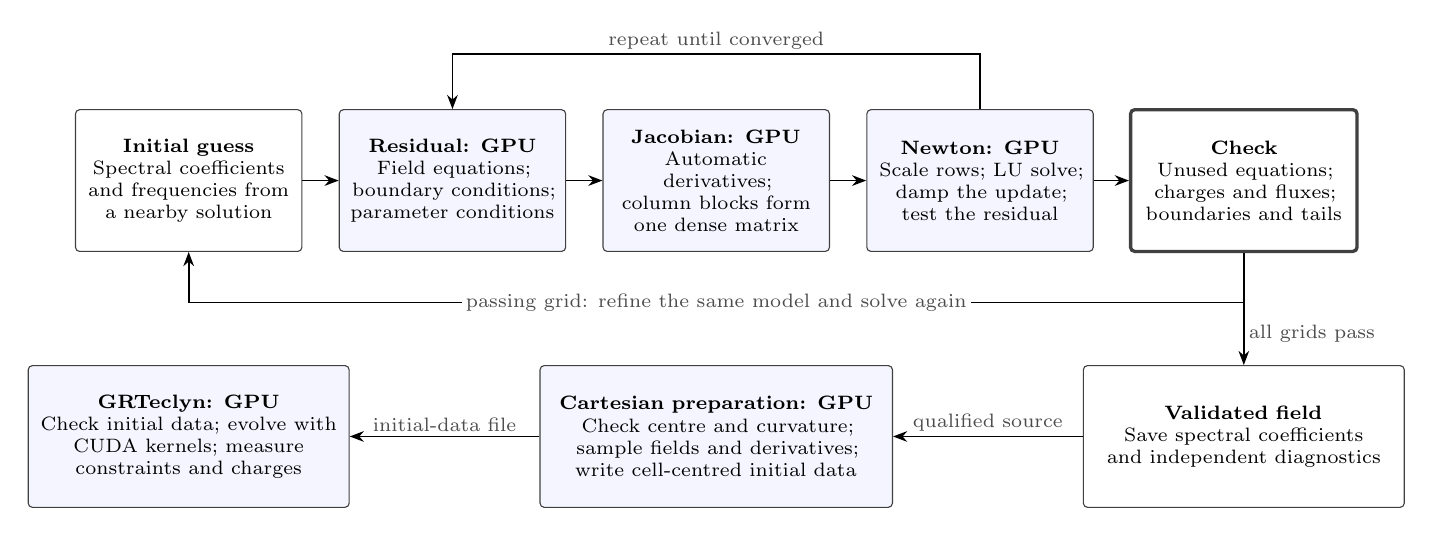
\begin{tikzpicture}[
  font=\scriptsize,
  box/.style={draw=black!75,rounded corners=1.5pt,align=center,
    text width=27mm,minimum height=18mm,inner sep=2.5pt},
  gpu/.style={box,fill=blue!4},
  check/.style={box,line width=1.2pt},
  flow/.style={-{Stealth[length=1.8mm]},line width=0.6pt},
  tag/.style={font=\scriptsize,text=black!70,fill=white,inner sep=1.5pt}]
\node[box] (guess) at (0,0) {\textbf{Initial guess}\\
  Spectral coefficients\\and frequencies from\\a nearby solution};
\node[gpu] (residual) at (3.35,0) {\textbf{Residual: GPU}\\
  Field equations;\\boundary conditions;\\parameter conditions};
\node[gpu] (jacobian) at (6.7,0) {\textbf{Jacobian: GPU}\\
  Automatic derivatives;\\column blocks form\\one dense matrix};
\node[gpu] (newton) at (10.05,0) {\textbf{Newton: GPU}\\
  Scale rows; LU solve;\\damp the update;\\test the residual};
\node[check] (check) at (13.4,0) {\textbf{Check}\\
  Unused equations;\\charges and fluxes;\\boundaries and tails};
\draw[flow] (guess) -- (residual);
\draw[flow] (residual) -- (jacobian);
\draw[flow] (jacobian) -- (newton);
\draw[flow] (newton) -- (check);
\draw[flow] (newton.north) -- ++(0,7mm) -|
  node[tag,pos=0.25,above] {repeat until converged} (residual.north);
\draw[flow] (check.south) -- (13.4,-1.55) -- (0,-1.55) -- (guess.south);
\node[tag] at (6.7,-1.55) {passing grid: refine the same model and solve again};
\node[box,text width=39mm] (save) at (13.4,-3.25) {\textbf{Validated field}\\
  Save spectral coefficients\\and independent diagnostics};
\node[gpu,text width=43mm] (export) at (6.7,-3.25) {\textbf{Cartesian preparation: GPU}\\
  Check centre and curvature;\\sample fields and derivatives;\\write cell-centred initial data};
\node[gpu,text width=39mm] (evolve) at (0,-3.25) {\textbf{GRTeclyn: GPU}\\
  Check initial data; evolve with\\CUDA kernels; measure\\constraints and charges};
\draw[flow] (13.4,-1.55) -- node[tag,right] {all grids pass} (save.north);
\draw[flow] (save) -- node[tag,above] {qualified source} (export);
\draw[flow] (export) -- node[tag,above] {initial-data file} (evolve);
\end{tikzpicture}
\caption{Stationary solution and Cartesian evolution workflow. Thin boxes
construct or evolve fields; the heavy box tests equations and charges
independently of the solve. Blue boxes identify the main GPU calculations;
the host controls iteration and file output. Only passing stationary and
Cartesian-origin checks permit preparation of evolution data.}
\label{fig:solver}
\end{figure*}

\begin{table*}[t]
\caption{Setup of the principal experiments. Spectral grids list radial
and angular degrees; Cartesian grids list cells per spatial direction.
The mass $m$ fixes units, and particle endpoints use the coordinate $z$.}
\label{tab:setup}
\begin{ruledtabular}
\begin{tabular}{llll}
Model & Matter parameters & Resolutions & Role\\
\hline
E & Single field, $k=+1$ & $\clmErgoGridA/\clmErgoGridB/\clmErgoGridC$ & Stationary ergoregion\\
C & Independent fields, $k_1=+1$, $k_2=\clmOuterWinding$ &
 $\clmPairGridA/\clmPairGridB/\clmPairGridC$ & Counter-rotation and channel\\
P & Single field, $\omega/m=\clmTransportFrequency$ &
 $\clmParticleGridA/\clmParticleGridB/\clmParticleGridC$ & Axial spin selection\\
U & Single field, $\omega/m=\clmEvolutionFrequency$ &
 $\clmGridLow^3/\clmGridMid^3/\clmGridHigh^3$ & Evolution through $mt=\clmEndTime$\\
\end{tabular}
\end{ruledtabular}
\end{table*}

\section{Stationary solutions and initial data}
\label{sec:initial}

\subsection{Construction and independent validation}

Figure~\ref{fig:solver} separates the stationary solve from its independent
checks and the subsequent spacetime evolution. A host process selects the
graphics processing unit (GPU) and enables double precision before JAX
compiles the field residual. The compiled residual and its automatically
differentiated Jacobian execute on the GPU. Jacobian columns are evaluated
in blocks to limit temporary memory, while the assembled dense matrix remains
on the device for LU factorization, the Newton correction and line-search
residual evaluations. Here LU denotes triangular matrix factorization.

A tensor-product Chebyshev representation covers a compactified radial
coordinate and the polar angle. Analytic factors remove the scalar's known
axis and parity behavior before Newton iteration solves for the remaining
smooth functions and frequencies. Asymptotic flatness fixes the time
normalization. For the counter-rotating pair, one scalar amplitude is adjusted
to make the total angular momentum vanish.

Every reported stationary model passes three independently recovered
resolutions. The checks include Einstein equations not used in the solve,
the Klein--Gordon equations evaluated in both intrinsic and Cartesian
coordinates, boundary conditions, spectral tails and independently evaluated
volume and surface charges. A small Newton residual alone is insufficient:
the equations not used by the solver must also hold.



\subsection{Cartesian initial data}

For evolution we evaluate the stationary metric and both real scalar
components at the Cartesian cell centres. The lapse $\alpha$, shift
$\beta^i$ and spatial metric $\gamma_{ij}$ are defined by
\begin{equation}
 ds^2=-\alpha^2dt^2+\gamma_{ij}(dx^i+\beta^idt)(dx^j+\beta^jdt),
 \label{eq:threeplusone}
\end{equation}
with $\alpha=e^{f/2}$ and $\beta^\varphi=-w$ for Eq.~\eqref{eq:metric}.
Spatial indices are $i,j$. Metric derivatives determine the extrinsic
curvature before sampling. The complex evolution field is
$\Phi=\chi/\sqrt{4\pi}$, with normal momentum
$\Pi=n^\mu\partial_\mu\Phi$, where $n^\mu$ is the future unit normal to a
constant-time slice. A local Cartesian polynomial representation supplies
regular derivatives at the centre and is checked against the field equations
and curvature before interpolation.

\begin{figure*}[t]
\centering
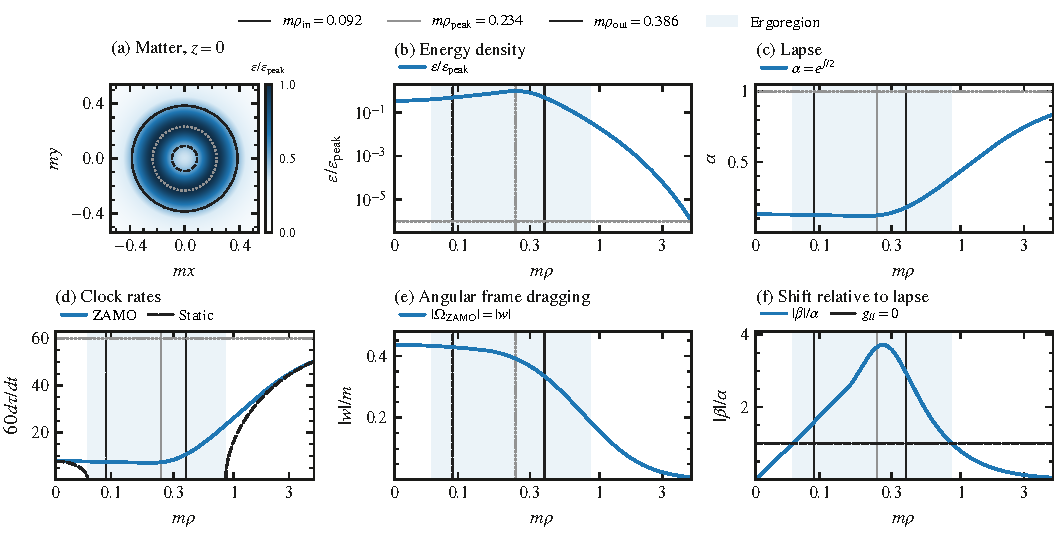
\includegraphics[width=\textwidth,height=0.38\textheight,keepaspectratio]{particles/ergoregion-372-cross-section.pdf}
\caption{Equatorial matter, density, lapse, clock rates, angular dragging
and shift/lapse ratio for a compact single ring, against coordinate position
or radius. Vertical lines mark the density peak and half-peak crossings;
shading marks the ergoregion. The metric supports an ergoregion across the
matter distribution and its surrounding tail.}
\label{fig:ergo}
\end{figure*}

\section{Numerical setup}
\label{sec:numerics}

Table~\ref{tab:setup} separates the physical models from the experiments
performed on them. The stationary ergoregion examples, particle backgrounds
and evolved ring are distinct configurations.



The Cartesian evolutions use GRTeclyn~\cite{grteclyn}, the conformal covariant
Z4 formulation (CCZ4), fourth-order spatial derivatives and fourth-order
Runge--Kutta time integration. The initial stationary lapse and shift evolve
with $1+\log$ slicing and a Gamma-driver shift condition. The uniform cube
has side length $mL=\clmBoxLength$, with time step
$\Delta t/\Delta x=\clmTimeStep$ and Sommerfeld conditions on each outer
face. Constraint norms use the same interior sphere, $mr<\clmInteriorRadius$,
at every resolution. These choices define the short-time comparison.

Particle integrations use two Runge--Kutta tolerances, spin reversal and
simultaneous background/spin reversal. An independent axial first-integral
calculation checks the near-turning trajectories. Appendix~\ref{app:checks}
collects the principal numerical tolerances.

\begin{figure*}[t]
\centering
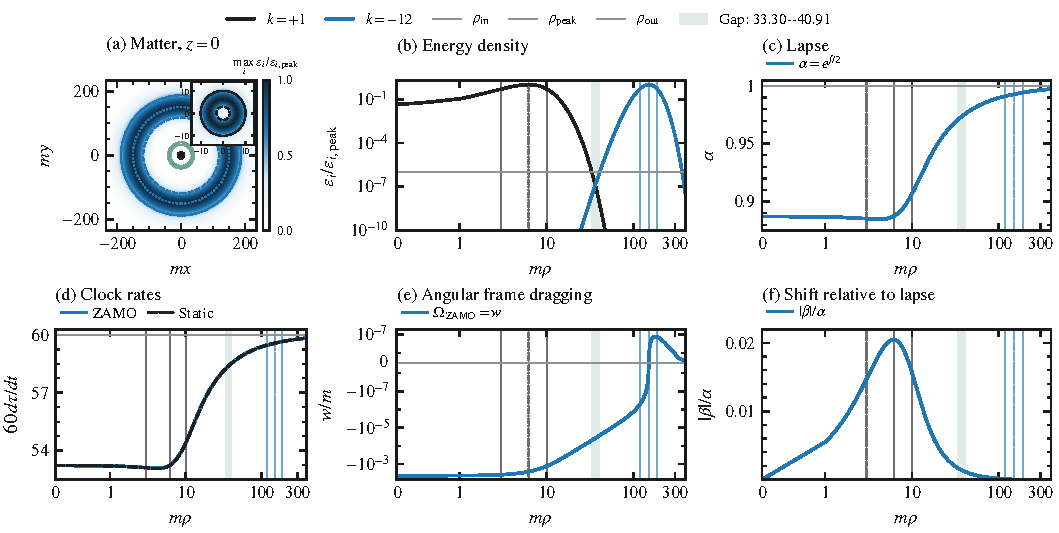
\includegraphics[width=\textwidth,height=0.38\textheight,keepaspectratio]{two-rings/annular-cross-section.pdf}
\caption{Equatorial matter distribution, component densities, lapse,
clock rates, signed angular dragging and shift/lapse ratio for the
counter-rotating pair. Black and blue distinguish the scalar components;
vertical lines mark half-peak crossings and peaks, and green marks the
low-density interval. Zero total angular momentum retains local frame dragging.}
\label{fig:channel}
\end{figure*}

\section{Diagnostics and criteria}
\label{sec:diagnostics}

\subsection{Ergoregions and frame dragging}

The stationary Killing vector is $\partial_t$. Its squared norm is
\begin{equation}
 g_{tt}=-\alpha^2+\gamma_{\varphi\varphi}w^2
       =\alpha^2(\mathcal{D}^2-1),\qquad
 \mathcal{D}=\frac{\sqrt{\gamma_{ij}\beta^i\beta^j}}{\alpha}.
 \label{eq:ergo}
\end{equation}
An ergoregion requires $g_{tt}>0$, consistently resolved across the stationary
grids. The dimensionless ratio $\mathcal{D}$ compares the shift norm with the
lapse. It is a metric diagnostic; a local observer measures light speed $c$.
A zero-angular-momentum observer (ZAMO) rotates at angular velocity $w$.
A clock held at fixed coordinates instead has rate
$d\tau/dt=\sqrt{-g_{tt}}$ wherever that observer is timelike.

\subsection{Angular momentum and the low-density channel}

For the phase convention in Eq.~\eqref{eq:phase}, the scalar charges obey
\begin{equation}
 \begin{split}
 Q_a&=\frac{1}{4\pi}\int
       \frac{(\omega_a+k_aw)A_a^2}{\alpha}\,dV,\\
 J_a&=-k_aQ_a,\qquad J=\sum_aJ_a,
 \end{split}
 \label{eq:charges}
\end{equation}
where $dV$ is proper spatial volume, $Q_a$ is the Noether charge and $J_a$
the component angular momentum. Independent surface measurements test $J$.
The asymptotic coefficient $w\sim2J/r^3$ fixes only the leading exterior
rotational term; cancelling it allows nonzero interior dragging.

Let $\epsilon_a=T^{(a)}_{\mu\nu}n^\mu n^\nu$ be the Eulerian energy density
of component $a$, with stress tensor $T^{(a)}_{\mu\nu}$. Its relative density is
\begin{equation}
 \eta_a(\rho,z)=\frac{\epsilon_a(\rho,z)}{\epsilon_{a,\mathrm{peak}}},
 \qquad \eta_a<\clmDensityCutoff\quad\hbox{for each component},
 \label{eq:density}
\end{equation}
where $\epsilon_{a,\mathrm{peak}}$ is that component's equatorial peak.
The last outer crossing for the inner field and the first inner crossing for
the outer field define the equatorial interval. We then test a common
finite-height tube and the density along every particle trajectory.
This definition retains the diffuse scalar tails.

\subsection{Equal-energy particle comparisons}

A Killing vector $\xi^\mu$ supplies a conserved particle quantity,
\begin{equation}
 C_\xi=p_\mu\xi^\mu+\frac12S^{\mu\nu}\nabla_\mu\xi_\nu,
 \qquad E=-C_{\partial_t},
 \label{eq:energy}
\end{equation}
where $E$ includes the spin contribution. All compared launches have equal
$E$ and unit particle rest mass. Passage means reaching the specified
finite target before a first turnaround while preserving particle invariants
and the timelike and supplementary conditions. Spin selection requires
opposite orientations to give different endpoints under tolerance changes
and independent timing checks.

\begin{figure*}[t]
\centering
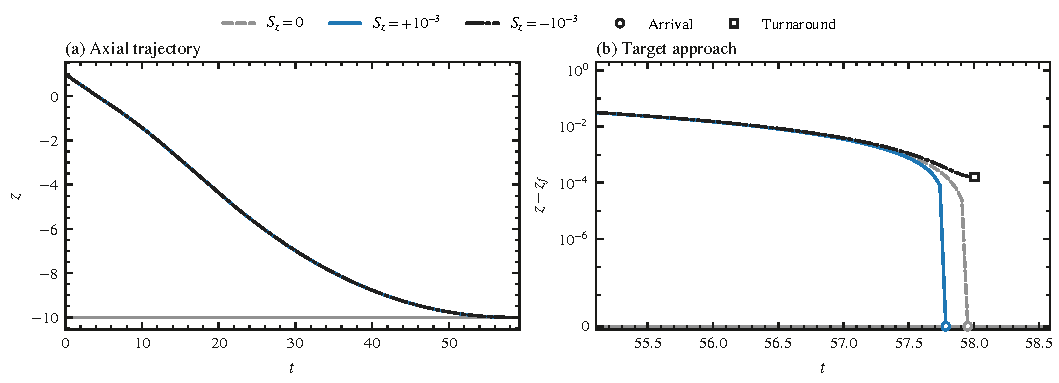
\includegraphics[width=\textwidth,height=0.36\textheight,keepaspectratio]{particles/strong-uphill-073.pdf}
\caption{Axial coordinate against time and distance from the target
against time for equal-energy particles in the single-ring background.
Grey, blue and black denote zero, positive and negative axial spin;
circles mark arrivals and the square marks a first turnaround.
Reversing the spin changes arrival into turnaround near the finite target.}
\label{fig:selection}
\end{figure*}

\section{Single rings with ergoregions}
\label{sec:ergo}

Compact single-ring solutions contain a resolved region with $g_{tt}>0$.
Figure~\ref{fig:ergo}(a,b) relates its position to the matter density;
panels (c,d) show the lapse and the two observer clock rates. Panels (e,f)
distinguish angular frame dragging from $\mathcal{D}$. Static observers cease
to be timelike inside the shaded region, while the ZAMO clock remains
well defined.

The strongest independently verified example has
$\mathcal{D}_{\max}\simeq\clmBestDragging$. This is the largest accepted
value in the sampled stationary family. Table~\ref{tab:results} gives a
separate quantitative example for the model plotted in Fig.~\ref{fig:ergo}.



\begin{table*}[t]
\caption{Representative measured results. Lengths and times use the scalar
mass unit; $E$ is the spin-corrected energy of a unit-rest-mass particle.
The dragging maximum and the plotted ergoregion example refer to distinct
stationary configurations.}
\label{tab:results}
\begin{ruledtabular}
\begin{tabular}{lll}
Experiment & Quantity & Measurement\\
\hline
Strongest sampled single ring & $\mathcal{D}_{\max}$ & $\clmBestDragging$\\
Plotted ergoregion ring & $\max g_{tt}$ & $\clmErgoGtt$\\
Counter-rotating pair & $J_1$, $J_2$ & $\clmInnerJ$, $\clmOuterJ$\\
Counter-rotating pair & $m\rho$ interval & $[\clmGapInner,\clmGapOuter]$\\
Between-ring transport & $E$ & $\clmTransitEnergy$\\
Between-ring transport & $mz_{\mathrm{launch}}\to mz_{\mathrm{target}}$ & $\clmLaunchZ\to\clmTargetZ$\\
Between-ring transport & $m(t_+-t_-)$ & $\clmTransitSplit$\\
Axial single-ring transport & $E$ & $\clmSelectionEnergy$\\
Axial single-ring transport & $mz_{\mathrm{turn}}$ for negative spin & $\clmTurnZ$\\
Evolution at $mt=\clmEndTime$ & Hamiltonian order, finer pair & $\clmHamOrder$\\
Evolution at $mt=\clmEndTime$ & Momentum order, finer pair & $\clmMomOrder$\\
Evolution at $mt=\clmEndTime$ & Charge-change self-convergence order & $\clmChargeOrder$\\
\end{tabular}
\end{ruledtabular}
\end{table*}

\section{Counter-rotating rings and a low-density channel}
\label{sec:channel}

Two independent fields with opposite winding form concentric rings whose
component angular momenta cancel. The volume and infinity measurements of
the total angular momentum agree within the independent numerical checks.
Nevertheless, the angular frame dragging is nonzero in the interior.

Figure~\ref{fig:channel}(a,b) shows the spatial separation and the
component-normalized density profiles. Both satisfy Eq.~\eqref{eq:density}
in the shaded interval, whose width is $m\Delta\rho\simeq\clmGapWidth$.
Panels (c,d) show the lapse and clock rates. Panels (e,f) display the signed
dragging and shift/lapse ratio. The cancellation of the global angular
momentum therefore coexists with a resolved, locally rotating geometry.

All $\clmTransitTracks$ equal-energy particle tracks reached the opposite
finite-height endpoint while remaining inside the validated tube.
The controls include zero spin, both axial spin orientations and simultaneous
background/spin reversal at two tolerances. The maximum density encountered
along the trajectories remained below the component-wise cutoff.
The measured spin-dependent coordinate transit-time difference appears in
Table~\ref{tab:results}.



\begin{figure*}[t]
\centering
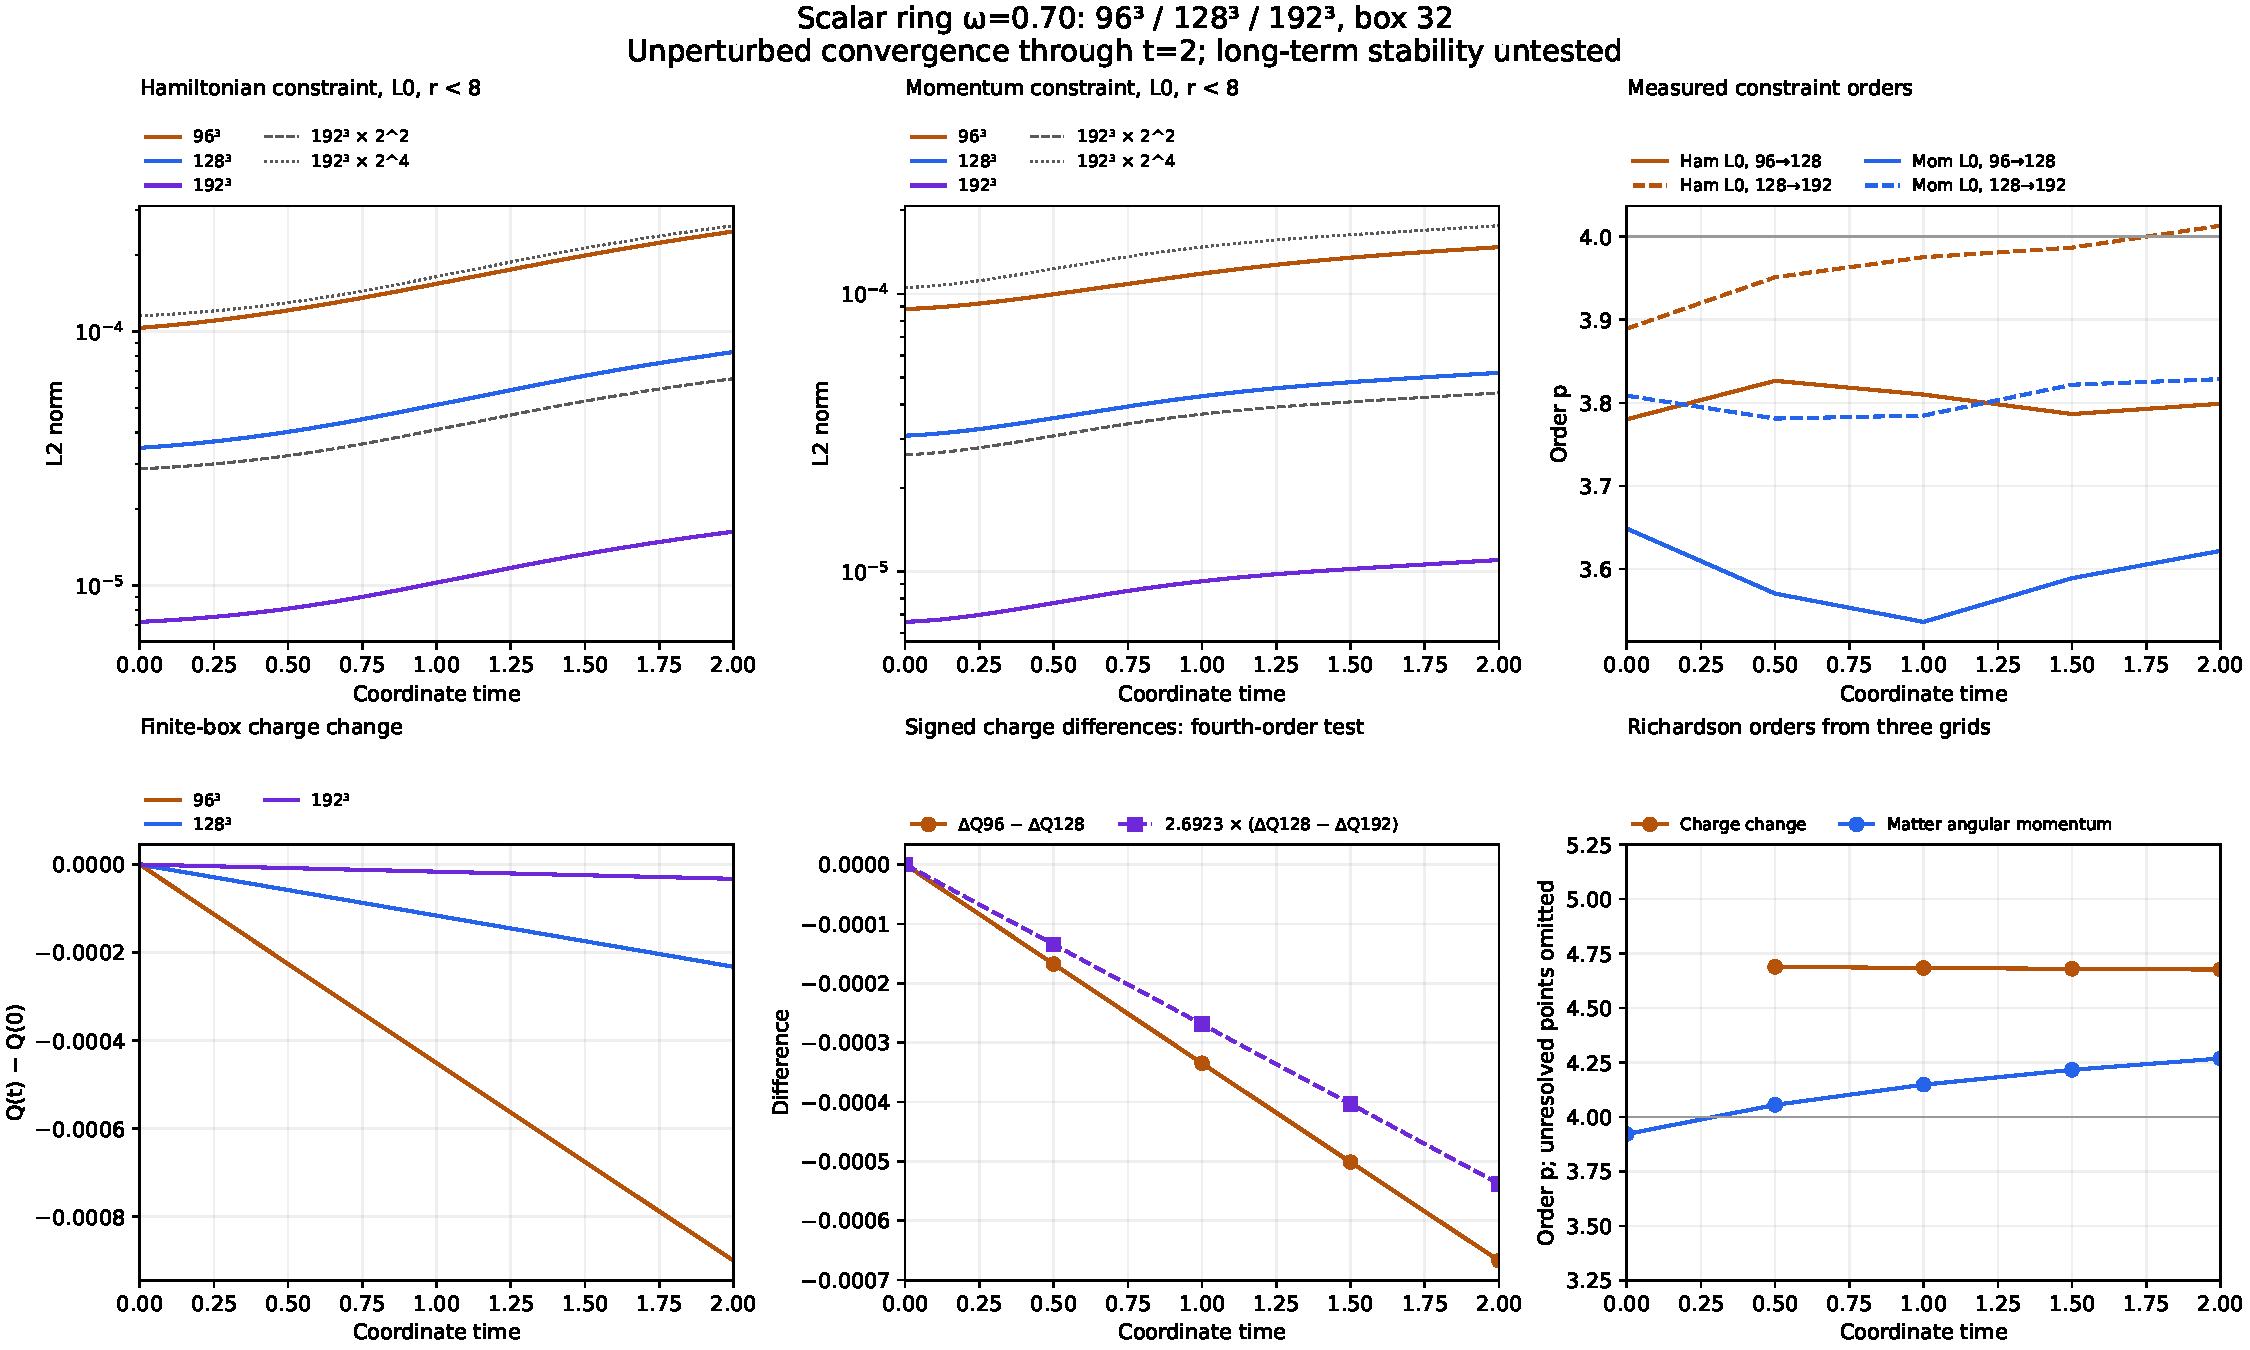
\includegraphics[width=\textwidth,height=0.38\textheight,keepaspectratio]{evolution/ring070-evolution-convergence.pdf}
\caption{Interior constraint norms, measured orders and charge changes
against time for three Cartesian resolutions. The legend identifies
resolutions, reference rescalings and adjacent-grid pairs; $D$ denotes the
charge-change difference in Eq.~\eqref{eq:richardson}. The constraint and
observable errors decrease consistently under refinement.}
\label{fig:convergence}
\end{figure*}

\section{Spin-dependent arrival and turnaround}
\label{sec:selection}

The axial single-ring experiment tests whether spin orientation changes
arrival at a prescribed target at fixed conserved energy. The ring's angular
momentum is negative. A particle with positive axial spin reaches the target,
whereas its negative-spin counterpart first turns just before it; the
zero-spin control reaches the target. Figure~\ref{fig:selection}(a) shows
the full trajectories, and panel (b) resolves their separation near the
endpoint. The target and spin magnitude are specified in
Table~\ref{tab:results} and the figure legend, where $S_z$ denotes the
signed axial particle spin in unit-rest-mass coordinates.

Independent first-integral quadratures reproduce the nonmarginal arrival
times, and direct substitution checks the reduced dynamics against the full
Cartesian particle equations. This establishes spin-dependent finite-target
selection in the stationary background.





\section{Short-time Cartesian evolution and convergence}
\label{sec:evolution}

The weaker single ring provides a short-time test of the Cartesian initial
data and spacetime evolution. Three uniform grids evolved the same
unperturbed stationary solution through $mt=\clmEndTime$.
Figure~\ref{fig:convergence}(a,b) shows decreasing interior constraint norms
and second- and fourth-order rescalings. Panel (c) gives the orders measured
between adjacent resolutions. Because the exact constraints vanish, their
norms can be compared directly under resolution rescaling.

The finer-pair constraint orders approach fourth order
(Table~\ref{tab:results}). Charge changes also decrease with resolution,
as shown in Fig.~\ref{fig:convergence}(d). Panels (e,f) compare the signed
charge differences and the inferred orders for charge change and matter
angular momentum. These are measured using the unequal grid spacings,
rather than assuming a fixed refinement ratio. Together these tests show
short-time numerical convergence for the evolved configuration.



\section{Conclusions}
\label{sec:conclusion}

Self-gravitating canonical scalar rings provide stationary geometries with
resolved ergoregions and spin-dependent test-particle transport. A pair of
counter-rotating fields retains local frame dragging despite cancellation of
its total angular momentum. Their separated density distributions leave a
finite-height, low-density channel traversed by the tested particles.
In the single-ring experiment, changing spin orientation at fixed conserved
energy changes arrival at a finite target into turnaround. The weaker ring's
Cartesian evolution exhibits short-time constraint and observable convergence.
These findings connect stationary field structure to finite-distance transport
within the specified matter and test-particle models.

\begin{acknowledgments}
This work was supported by Gravity Frontiers
(\url{https://www.gravityfrontiers.org/en}), which funded the underlying
research and the development of the numerical-simulation software. The authors
acknowledge the GRTL Collaboration for \texttt{GRChombo}, \texttt{GRTresna},
and \texttt{GRTeclyn}.
\end{acknowledgments}

\FloatBarrier
\appendix
\section{Notation}
\label{app:notation}

Spatial norms use $\gamma_{ij}$. The principal notation is collected below.
\begin{center}
\footnotesize
\begin{tabular}{@{}p{0.23\columnwidth}p{0.70\columnwidth}@{}}
\hline
Symbol & Meaning\\
\hline
$\chi_a,A_a,\omega_a,k_a$ & Scalar field, amplitude, frequency, winding\\
$m$ & Common scalar mass\\
$f,B,\nu,w$ & Stationary metric functions\\
$\rho,z$ & Cylindrical coordinates\\
$\alpha,\beta^i,\gamma_{ij}$ & Lapse, shift, spatial metric\\
$\mathcal{D}$ & Shift norm divided by lapse\\
$Q_a,J_a,J$ & Scalar charge, component and total spin\\
$\epsilon_a,\eta_a$ & Energy density and relative density\\
$p^\mu,u^\mu,S^{\mu\nu}$ & Particle momentum, velocity, spin tensor\\
$E,\tau$ & Conserved particle energy, proper time\\
$\Phi,\Pi$ & Evolution field and normal momentum\\
$h,p$ & Grid spacing and convergence order\\
$\Delta Q,D_{ab}$ & Charge change and its grid difference\\
\hline
\end{tabular}
\end{center}

\section{Independent validation and convergence estimates}
\label{app:checks}

The stationary equations and charge-flux comparisons use the tolerance
$\clmFieldTolerance$. Spectral tails, relative changes between stationary
resolutions and the matter-density cutoff are tested separately. Particle
mass, spin, conserved energy and supplementary-condition errors are required
to remain below $\clmInvariantTolerance$ in their stated normalization.
The independent nonmarginal timing comparison uses $\clmTimingTolerance$.
These are acceptance tolerances for the numerical tests, not error bars on
every derived physical observable.

For the Cartesian charge, let $Q_N(t)$ be the finite-box scalar charge at
resolution $N$, and $\Delta Q_N(t)=Q_N(t)-Q_N(0)$. With
$h_a>h_b>h_c$ the three grid spacings, define
\begin{equation}
 D_{ab}=\Delta Q_a-\Delta Q_b,\qquad
 \frac{D_{ab}}{D_{bc}}=
 \frac{h_a^p-h_b^p}{h_b^p-h_c^p}.
 \label{eq:richardson}
\end{equation}
The order $p$ is fitted from signed resolved differences. This assumes a
leading power-law error term; the resulting extrapolation is an asymptotic
estimate. The expected fourth-order difference factor for these grids is
$\clmFourthFactor$, the rescaling used in
Fig.~\ref{fig:convergence}(e).

% Expansion points: give the stationary elliptic equations and their boundary
% conditions, Cartesian origin representation, full particle velocity relation,
% and the detailed stationary/particle convergence tables in this appendix.

\section{Numerical data and figure provenance}
\label{app:data}

The accompanying repository stores stationary fields, portable evolution
diagnostics and the numerical inputs for the figures. Each stationary and
particle study retains its configuration, checks and checksums. The manuscript
number ledger links quoted measurements to specific archived diagnostic
entries; its checker verifies source hashes before generating the macros.
Figure assets are read directly from the repository's results directory.

\begin{thebibliography}{9}
\bibitem{kleihaus2005}
B. Kleihaus, J. Kunz and M. List,
``Rotating boson stars and Q-balls,''
\href{https://doi.org/10.1103/PhysRevD.72.064002}{Phys. Rev. D \textbf{72}, 064002 (2005)},
\href{https://arxiv.org/abs/gr-qc/0505143}{arXiv:gr-qc/0505143}.
\bibitem{kleihaus2008}
B. Kleihaus, J. Kunz, M. List and I. Schaffer,
``Rotating boson stars and Q-balls. II. Negative parity and ergoregions,''
\href{https://doi.org/10.1103/PhysRevD.77.064025}{Phys. Rev. D \textbf{77}, 064025 (2008)},
\href{https://arxiv.org/abs/0712.3742}{arXiv:0712.3742}.
\bibitem{song2023}
Y. Song, Y. Cen, L. Tang, J. Hu, K. Diao, X. Zhao and S. Shi,
``The particle surface of spinning test particles,''
\href{https://doi.org/10.1140/epjc/s10052-023-11970-5}{Eur. Phys. J. C \textbf{83}, 833 (2023)}.
\bibitem{grteclyn}
GRTL Collaboration, \emph{GRTeclyn},
\url{https://grtlcollaboration.github.io/GRTeclyn/}.
\end{thebibliography}
\end{document}
